\section{évaluation}
\label{sec:evaluation}

\subsection{WP1 : Impact du prétraitement}

\paragraph{Analyse qualitative.}
L'étude de l'impact des espaces de couleur (RGB, HSV, LAB), des filtres de lissage (Gaussien, Médian, Bilatéral, $k=5$) et des stratégies d'augmentation (color jitter, Random Erasing) est réalisée qualitativement. Ces expériences montrent visuellement que les filtres de lissage préservent la structure générale de la personne, et que l'augmentation par Random Erasing simule efficacement des occultations partielles.

\paragraph{Benchmark de résolution.}
Seule l'expérience quantitative de ce WP concerne l'impact de la résolution d'entrée (tableau \ref{tab:resolution}). Le modèle de référence est ResNet-50 entraîné à $256 \times 128$.

\begin{table}[t]
\centering
\caption{Impact de la résolution d'entrée sur les performances Re-ID (ResNet-50, Market-1501).}
\label{tab:resolution}
\begin{tabular}{lcccc}
\toprule
Résolution & Rank-1 & Rank-5 & Rank-10 & mAP \\
\midrule
$256\times128$ (base) & 77,40 & 90,11 & 93,38 & 54,47 \\
$128\times64$         & 77,40 & 90,11 & 93,38 & 54,47 \\
$64\times32$          & 65,02 & 82,57 & 87,77 & 44,27 \\
$32\times16$          & 32,57 & 52,35 & 60,57 & 21,38 \\
\bottomrule
\end{tabular}
\end{table}

La résolution de $256 \times 128$ et $128 \times 64$ donnent des résultats identiques, suggérant que le réseau est robuste à un facteur de réduction 2. Une dégradation significative n'apparaît qu'à $64 \times 32$ (Rank-1 $-12,4$ pp), et est catastrophique à $32 \times 16$ ($-44,8$ pp), o\`{u} les détails discriminants sont irrémédiablement perdus.

\subsection{WP2 : Descripteurs classiques vs. profonds}

Le tableau \ref{tab:classical_vs_deep} compare les descripteurs classiques à notre modèle profond de référence.

\begin{table}[t]
\centering
\caption{Comparaison des descripteurs classiques et profonds sur Market-1501.}
\label{tab:classical_vs_deep}
\resizebox{\columnwidth}{!}{
\begin{tabular}{lcccc}
\toprule
Descripteur & Rank-1 & Rank-5 & Rank-10 & mAP \\
\midrule
HOG \cite{dalal2005histograms}                 & 0,68  & 2,46  & 3,89  & 0,38 \\
Hist. couleur                                  & 1,87  & 4,33  & 7,07  & 0,69 \\
SIFT$^\dagger$ \cite{lowe2004distinctive}      & 0,50  & 7,50  & 14,50 & 2,51 \\
\midrule
ResNet-50 (profond)                            & 77,40 & 90,56 & 93,62 & 55,58 \\
ResNet-50 + Re-ranking \cite{zhong2017re}      & \textbf{80,29} & 91,03 & 93,82 & \textbf{65,04} \\
\bottomrule
\end{tabular}
}
\vspace{1pt}
\footnotesize{$^\dagger$ évalué sur un sous-ensemble ($n{=}200$ requêtes, $n{=}1\,000$ galerie).}
\end{table}

L'écart entre descripteurs classiques et profonds est drastique: le meilleur descripteur classique (histogramme de couleur) ne dépasse pas 1,87\,\% en Rank-1, soit 75 points de pourcentage de moins que ResNet-50. Cela s'explique par l'incapacité des descripteurs à la main à généraliser aux variations intra-classe (illumination, pose). Curieusement, SIFT obtient un Rank-10 de 14,50\,\% mais un Rank-1 très faible (0,50\,\%), ce qui indique que ses correspondances correctes se situent généralement plus loin dans le classement. Le re-ranking améliore le ResNet-50: la mAP gagne $+9,5$ pp (55,58 $\to$ 65,04), confirmant l'intérêt de la ré-estimation de voisinage k-réciproque.

\subsection{WP4 : Ablation des stratégies de gel}

\begin{table}[t]
\centering
\caption{Comparaison des trois stratégies de gel sur Market-1501.}
\label{tab:ablation}
\resizebox{\linewidth}{!}{%
\begin{tabular}{lrrccc}
\toprule
Stratégie & Params train. & \% & Rank-1 & mAP & Temps \\
\midrule
Feature Extraction  & 1,54M &  6,2 &  7,07 &  2,33 &  9,9 min \\
Partial Fine-Tuning & 23,6M & 94,2 & 83,43 & 62,11 & 21,7 min \\
Full Fine-Tuning    & 25,0M & 100  & \textbf{85,36} & \textbf{66,33} & 28,4 min \\
\bottomrule
\end{tabular}}
\end{table}

\begin{figure}[t]
  \centering
  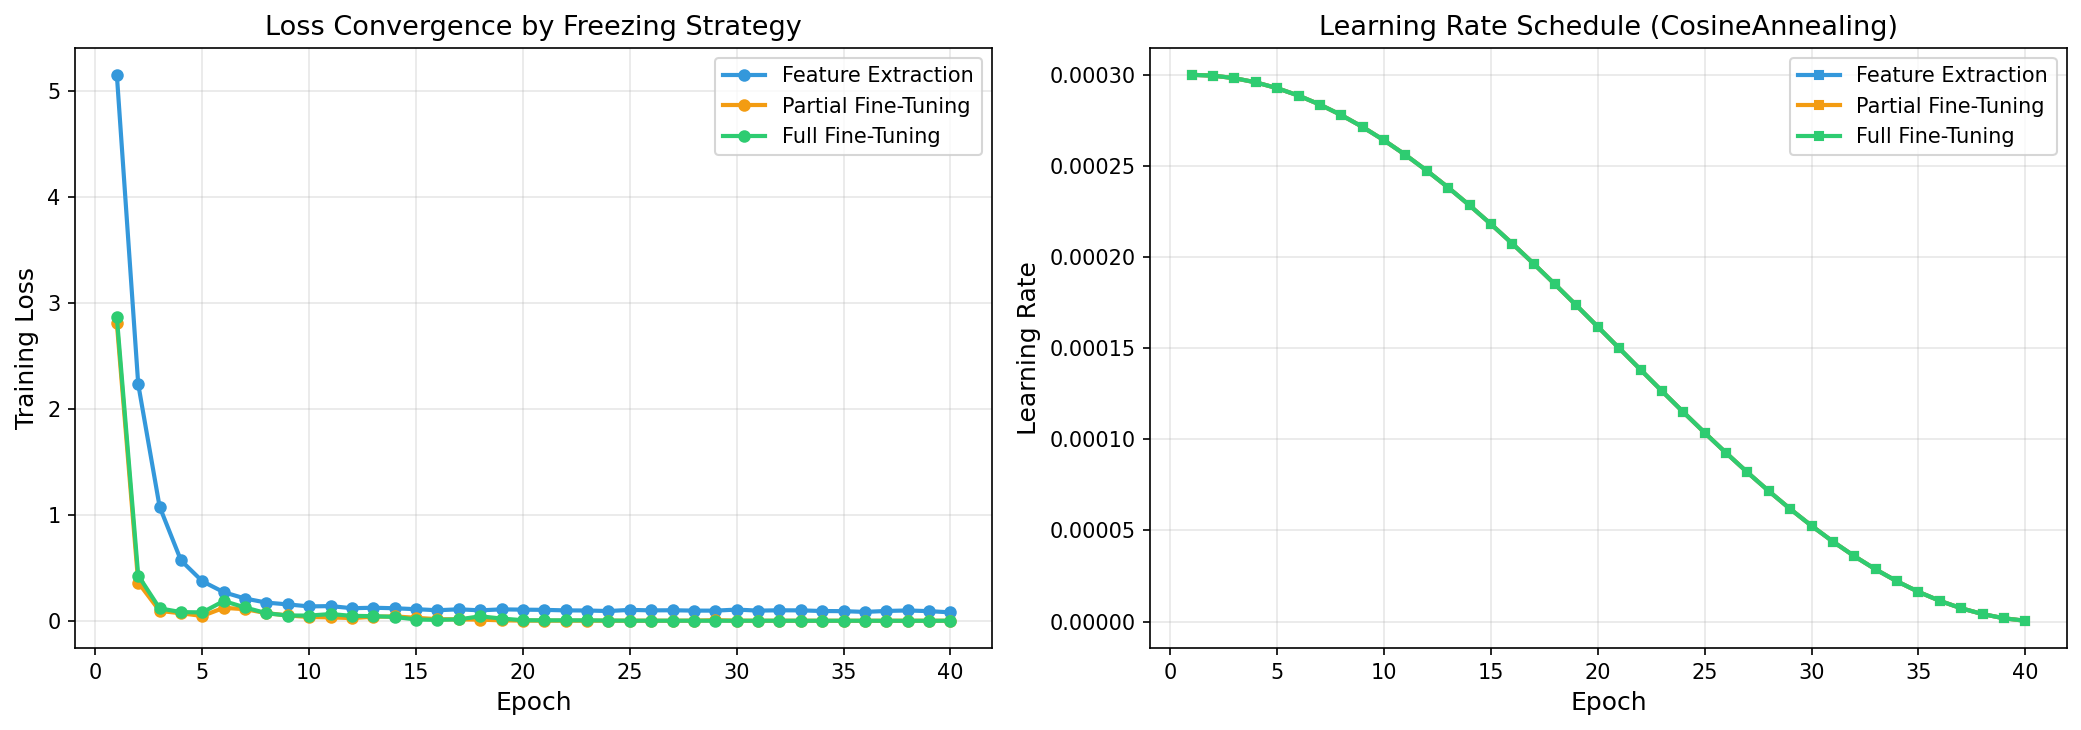
\includegraphics[width=\linewidth]{results/ablation_loss_curves.png}
  \caption{Courbes de perte pendant l'entraînement pour les trois stratégies de gel. Le gel total du backbone (Feature Extraction) atteint un plancher bien supérieur aux deux autres stratégies.}
  \label{fig:ablation_loss}
\end{figure}

Les résultats du tableau \ref{tab:ablation} et des courbes de figure \ref{fig:ablation_loss} montrent clairement que le gel total du backbone est catastrophique pour le Re-ID : les features ImageNet ne sont pas adaptées à la discrimination fine d'identités, et les 1,54M de paramètres entraînables (BN-Neck + classifieur) sont insuffisants pour surmonter ce déficit. Le fine-tuning partiel récupère l'essentiel de la performance ($+76$ pp par rapport au gel total) en libérant les couches hautes du réseau. Le fine-tuning complet apporte un gain supplémentaire de $+1,93$ pp en Rank-1 et $+4,22$ pp en mAP, au prix de $+6,7$ min d'entraînement -- un compromis favorable étant donné la disponibilité d'un GPU.

\subsection{WP5 : Comparaison architecturale ResNet-50 vs ViT}

\begin{table}[t]
\centering
\caption{Comparaison CNN/Transformer sur Market-1501. La latence est mesurée par image sur GPU.}
\label{tab:arch_comparison}
\resizebox{\linewidth}{!}{%
\begin{tabular}{lcc}
\toprule
Métrique & ResNet-50 & ViT-Base/16 \\
\midrule
Paramètres & 25,1M & 86,4M \\
FLOPs & 4,05 G & 6,46 G \\
Latence (ms/img) & 13,0 $\pm$ 0,6 & 10,7 $\pm$ 0,6 \\
Résolution & $256\times128$ & $224\times224$ \\
Dim. embedding & 2048 & 768 \\
\midrule
Rank-1 (\%) & 84,41 & \textbf{88,63} \\
mAP (\%) & 64,47 & \textbf{73,84} \\
Temps d'entraînement & $\sim$40 min & 47,9 min \\
\bottomrule
\end{tabular}}
\end{table}

\begin{figure}[t]
  \centering
  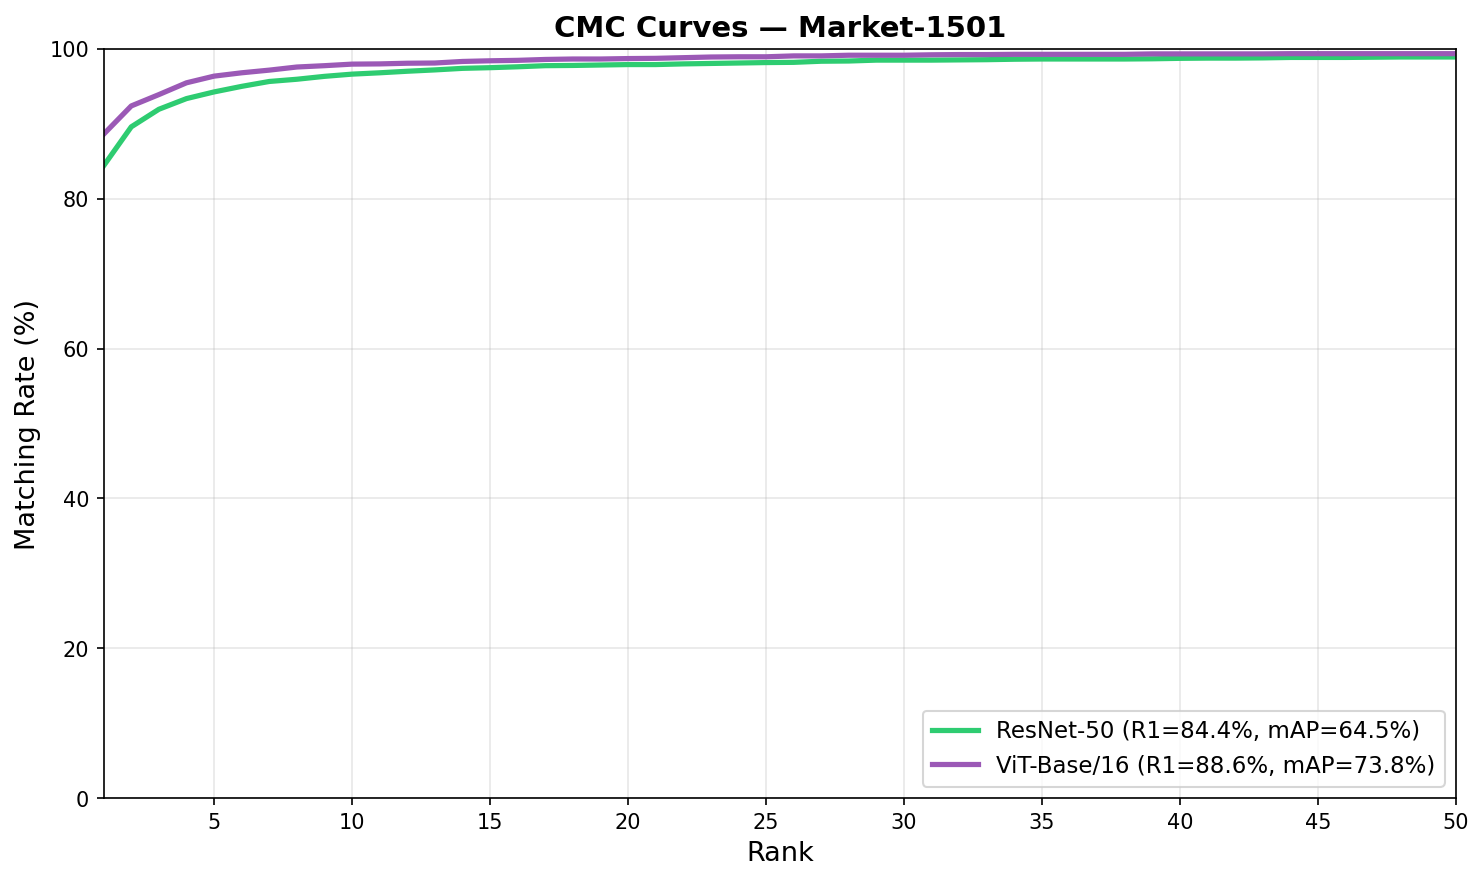
\includegraphics[width=\linewidth]{results/architecture_cmc_curves.png}
  \caption{Courbes CMC pour ResNet-50 et ViT-Base/16 sur Market-1501. ViT domaine à tous les rangs.}
  \label{fig:cmc_curves}
\end{figure}

Comme le montrent le tableau \ref{tab:arch_comparison} et la figure \ref{fig:cmc_curves}, ViT-Base/16 surpasse ResNet-50 sur tous les critères de qualité Re-ID : Rank-1 $+4,2$ pp, Rank-5 $+2,1$ pp, mAP $+9,4$ pp. Paradoxalement, ViT est plus rapide à l'inférence (10,7\,ms vs 13,0\,ms), car la convolution large du réseau est remplacée par des opérations matrice/vecteur efficacement parallélisables sur GPU. En revanche, ViT est 3,45$\times$ plus volumineux (86,4M vs 25,1M paramètres) et nécessite $\sim$20\,\% de temps d'entraînement supplémentaire. L'attention globale du Transformer lui permet de capturer des relations entre parties du corps spatialement distantes, ce qui se traduit par une meilleure séparation inter-classe dans l'espace d'embedding.

\subsection{WP6 : Adaptation de domaine}

\paragraph{Gap de domaine.}
Avant tout fine-tuning, nous mesurons le gap entre Market-1501 (source) et le dataset personnel (cible) à l'aide de la distance centraîde ($d_c = 0{,}603$), la similarité cosinus entre les centroids ($0{,}077$), et la MMD linéaire ($0{,}367$). Ces indicateurs confirment un décalage significatif entre les deux domaines, bien que les embeddings pré-entraînés se généralisent partiellement.

\paragraph{Résultats.}
\begin{table}[t]
\centering
\caption{Résultats d'adaptation de domaine (dataset cible : personnel). La mAP est la métrique principale en raison d'un artéfact d'évaluation sur un petit dataset (voir texte). Les Rank-1 et mAP du modèle source sont mesurés sur Market-1501.}
\label{tab:domain_adaptation}
\begin{tabular}{lcc}
\toprule
Expérience & Rank-1 & mAP \\
\midrule
Modèle source (Market-1501)  & 84,41 & 64,47 \\
Zero-Shot $\to$ Cible            & 100,00$^*$ & 78,27 \\
Transfer Learning $\to$ Cible    & 100,00$^*$ & \textbf{89,93} \\
\bottomrule
\end{tabular}
\vspace{2pt}
\footnotesize{$^*$ Rank-1 saturé : les images requêtes étant incluses dans la galerie, la correspondance exacte (sim. = 1) est toujours retournée en première position. La mAP (qui penalise le rang des \textit{autres} correspondances correctes) est plus représentative.}
\end{table}

\begin{figure}[t]
  \centering
  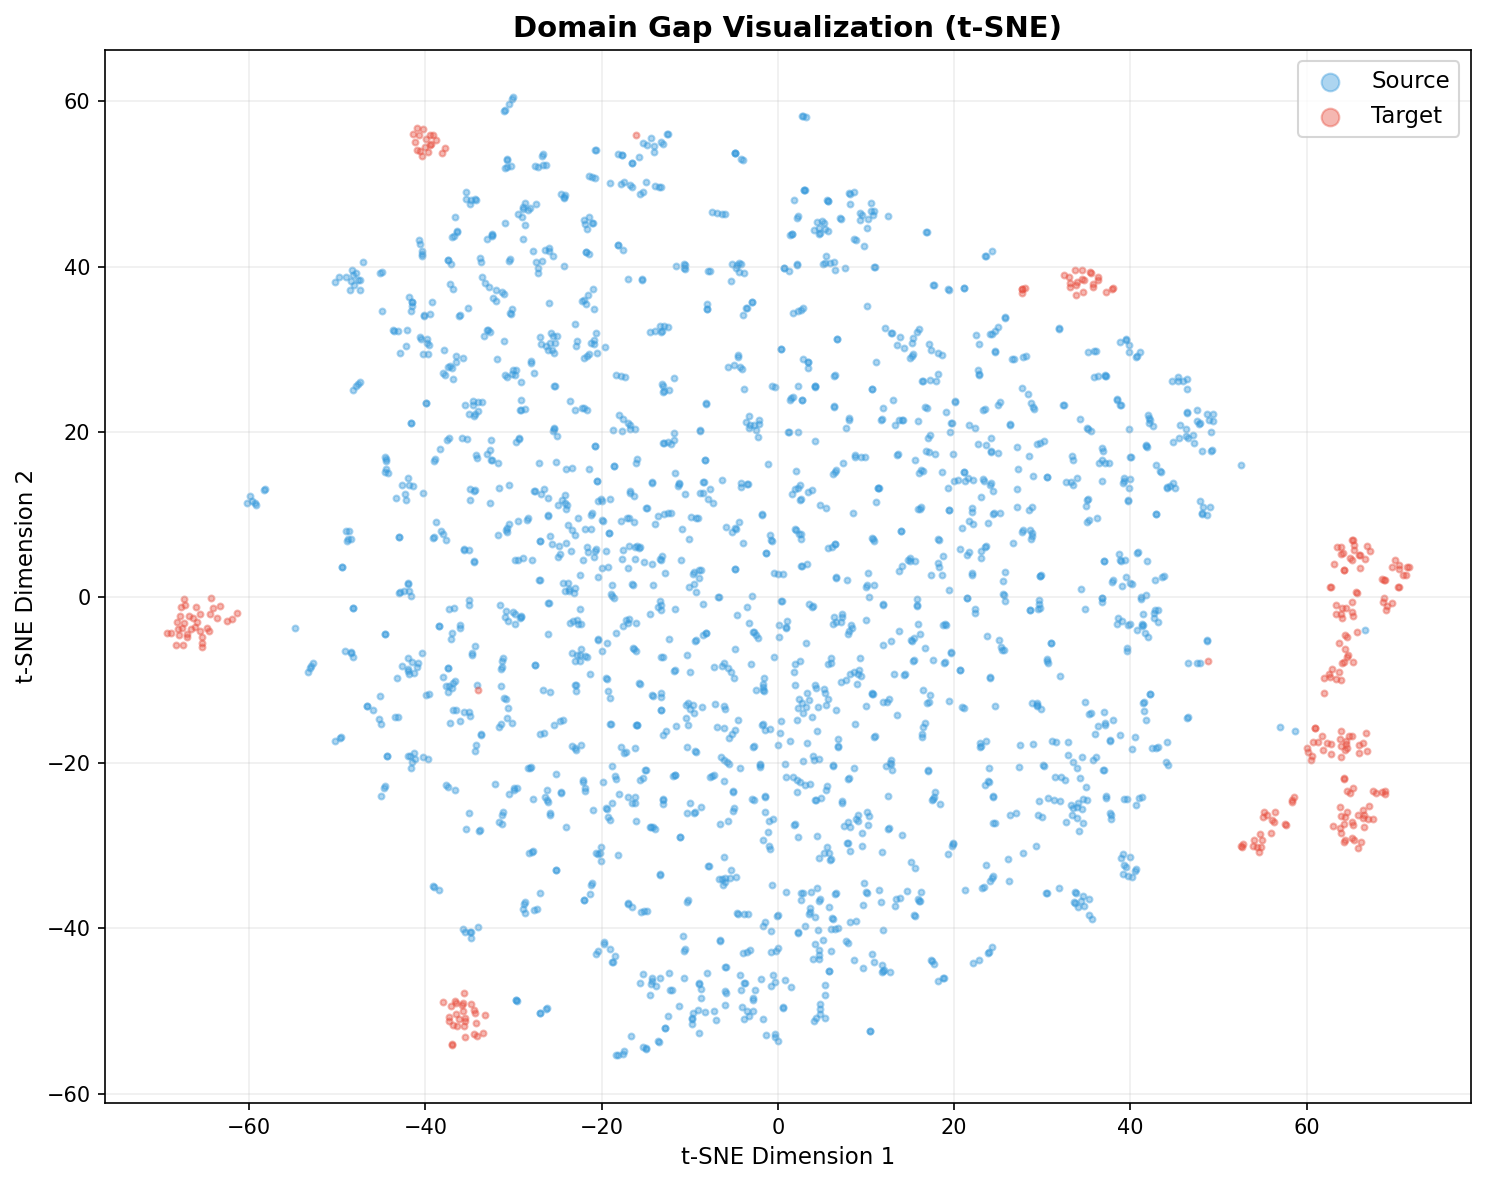
\includegraphics[width=\linewidth]{results/domain_gap_before_after.png}
  \caption{Visualisation t-SNE du gap de domaine avant et après adaptation. Après transfer learning, les embeddings du domaine cible s'organisent en clusters d'identité plus cohérents.}
  \label{fig:domain_gap}
\end{figure}

Le transfer learning (gel partiel, lr=$5 \times 10^{-5}$, 20 époques, 131 images) améliore la mAP de $+11,7$ pp (78,27 $\to$ 89,93\,\%). Cela démontre qu'un fine-tuning ciblé sur très peu de données (131 images) suffit à améliorer sensiblement la discrimination d'identité dans le domaine cible, même à partir d'un modèle entraîné sur un domaine différent.

\subsection{WP7 : Clustering d'albums}

\begin{table}[t]
\centering
\caption{Résultats du clustering DBSCAN ($\varepsilon = 0{,}18$) pour l'indexation automatique d'albums.}
\label{tab:clustering}
\resizebox{\columnwidth}{!}{
\begin{tabular}{lccc}
\toprule
Dataset & Pureté & Clusters & Imgs/cluster (moy.) \\
\midrule
Market-1501     & 88,95\,\% & 533 & 13,75 \\
Dataset personnel & \textbf{94,80\,\%} & \multicolumn{2}{c}{(eps optimal $\varepsilon \approx 0{,}15$)} \\
\bottomrule
\end{tabular}
}
\end{table}

La figure \ref{fig:domain_gap} (à gauche, identités source) illustre qualitativement la structuration des embeddings en clusters. DBSCAN est fortement sensible au seuil $\varepsilon$ : pour $\varepsilon \leq 0{,}15$, le nombre de clusters explose (plus de 500 pour Market-1501) fragmentant les identités ; pour $\varepsilon \geq 0{,}35$, l'effet de chaînage fusionne des identités distinctes en un seul mega-cluster (9 albums pour Market-1501 dont un de 12,804 images). Le pic de NMI et d'ARI, visible sur l'analyse de sensibilité, se situe à $\varepsilon \approx 0{,}2$ pour Market-1501 et $\varepsilon \approx 0{,}15$ pour le dataset personnel.

La pureté de 88,95\,\% sur Market-1501 (533 clusters, 13,75 images/cluster en moyenne, 191 images pour le plus grand) démontre que les embeddings ResNet-50 capturent efficacement l'identité plutôt que l'apparence brute -- le système gère les changements de pose et de caméra. Sur le dataset personnel (262 images, identités connues), la pureté atteint 94,80\,\%, confirmant la robustesse des features appris sur Market-1501 à un domaine différent.
